% THIS IS SIGPROC-SP.TEX - VERSION 3.1
% WORKS WITH V3.2SP OF ACM_PROC_ARTICLE-SP.CLS
% APRIL 2009
%
% It is an example file showing how to use the 'acm_proc_article-sp.cls' V3.2SP
% LaTeX2e document class file for Conference Proceedings submissions.
% ----------------------------------------------------------------------------------------------------------------
% This .tex file (and associated .cls V3.2SP) *DOES NOT* produce:
%       1) The Permission Statement
%       2) The Conference (location) Info information
%       3) The Copyright Line with ACM data
%       4) Page numbering
% ---------------------------------------------------------------------------------------------------------------
% It is an example which *does* use the .bib file (from which the .bbl file
% is produced).
% REMEMBER HOWEVER: After having produced the .bbl file,
% and prior to final submission,
% you need to 'insert'  your .bbl file into your source .tex file so as to provide
% ONE 'self-contained' source file.
%
% Questions regarding SIGS should be sent to
% Adrienne Griscti ---> griscti@acm.org
%
% Questions/suggestions regarding the guidelines, .tex and .cls files, etc. to
% Gerald Murray ---> murray@hq.acm.org
%
% For tracking purposes - this is V3.1SP - APRIL 2009

\documentclass{acm_proc_article-sp}

\begin{document}

\title{ACCELERATING GENETIC ALGORITHM PROCESSING FOR APPLICATION IN GAME ARTIFICIAL INTELLIGENCE}

%
% You need the command \numberofauthors to handle the 'placement
% and alignment' of the authors beneath the title.
%
% For aesthetic reasons, we recommend 'three authors at a time'
% i.e. three 'name/affiliation blocks' be placed beneath the title.
%
% NOTE: You are NOT restricted in how many 'rows' of
% "name/affiliations" may appear. We just ask that you restrict
% the number of 'columns' to three.
%
% Because of the available 'opening page real-estate'
% we ask you to refrain from putting more than six authors
% (two rows with three columns) beneath the article title.
% More than six makes the first-page appear very cluttered indeed.
%
% Use the \alignauthor commands to handle the names
% and affiliations for an 'aesthetic maximum' of six authors.
% Add names, affiliations, addresses for
% the seventh etc. author(s) as the argument for the
% \additionalauthors command.
% These 'additional authors' will be output/set for you
% without further effort on your part as the last section in
% the body of your article BEFORE References or any Appendices.

\numberofauthors{3} %  in this sample file, there are a *total*
% of EIGHT authors. SIX appear on the 'first-page' (for formatting
% reasons) and the remaining two appear in the \additionalauthors section.
%
\author{
% You can go ahead and credit any number of authors here,
% e.g. one 'row of three' or two rows (consisting of one row of three
% and a second row of one, two or three).
%
% The command \alignauthor (no curly braces needed) should
% precede each author name, affiliation/snail-mail address and
% e-mail address. Additionally, tag each line of
% affiliation/address with \affaddr, and tag the
% e-mail address with \email.
%
% 1st. author
\alignauthor
James C. Choa\\
       \affaddr{Department of Information Systems and Computer Science}\\
       \affaddr{Ateneo de Manila University}\\
       \email{choa.james@gmail.com}
% 2nd. author
\alignauthor
Holvin G. Tiu\\
       \affaddr{Department of Information Systems and Computer Science}\\
       \affaddr{Ateneo de Manila University}\\
       \email{nivloh3@yahoo.com}
\alignauthor
Walfrido David A. Diy
       \affaddr{Ateneo de Manila University}\\
       \email{wdiy@ateneo.edu}
}
% There's nothing stopping you putting the seventh, eighth, etc.
% author on the opening page (as the 'third row') but we ask,
% for aesthetic reasons that you place these 'additional authors'
% in the \additional authors block, viz.
% Just remember to make sure that the TOTAL number of authors
% is the number that will appear on the first page PLUS the
% number that will appear in the \additionalauthors section.

\maketitle
\begin{abstract}
Genetic algorithms have been applied to enhance Artificial Intelligence (AI) in
games. However, the biggest limiting factor in the use of genetic algorithms
has been the large amount of time it takes for an acceptable solution to evolve
after numerous generations. In light of this, we present a solution to speed up
the process by making use of the parallel computing capabilities of the Graphics
Processing Unit.
\end{abstract}

% A category with the (minimum) three required fields
\category{D.1.3}{Programming Techniques}{Concurrent Programming}[parallel programming]
%A category including the fourth, optional field follows...
\category{I.6.8}{Simulation and Modeling}{Types of Simulation}[parallel]

\terms{Graphics Processing Unit, Genetic Algorithm, Fitness function, Individual, Generation, Optimizer, Physical Time}

%%\keywords{ACM proceedings, \LaTeX, text tagging} % NOT required for Proceedings

\section{Introduction}
\subsection{Background of the Study}

% AI Game engine prog p 415
Genetic algorithms are one of the many types of artificial intelligence
techniques that exist today. If implemented well, genetic algorithms can
evolve a computer controlled agent to perform adequately according to some
set criteria defined in a fitness function. However, a significant amount of 
time is required for the algorithm to evolve a population of individual solutions 
into an acceptable solution \cite{Schwab04}. The time it takes can range from
a few hours to a number of weeks, depending on the complexity of the game where
the agent must perform. This limitation makes them difficult or impractical to
use in the process of game development \cite{Schwab04}.

% refer to the bottom part of p 415 and top part of p 417 in AI game engine prog
The primary reasons genetic algorithms take up a lot of time are the number of 
possible solutions that must be tested given a specific generation, the time it 
takes to evaluate each of these possible solutions, and the number of generations 
that may be needed before arriving at a single or a number of acceptable solutions \cite{Schwab04}. 
One way to tackle the issue is by using faster processors in order to reduce the
overall computation time of the genetic algorithm. A better solution would
be to process all the individuals in a single generation in parallel through the
use of threads. A computer processor is capable of a variety of things, but it is limited by its instruction throughput. Even with the modern CPU with multiple processing cores, the CPU can only
run one instruction at a time per core. This is where Graphics Processing Units, or GPUs, come in.
GPUs have been designed to execute a single set of instructions over numerous elements
of data, a technique known as ``Single-Instruction, Multiple-Thread \cite{pdf:NVCudaPrgGuide}.''
Not only do they have multiple processing units, each processing unit is also
capable of running several identical instructions simultaneously, making GPUs ideal
for highly parallel algorithms \cite{pdf:NVCudaPrgGuide}. It is our goal therefore to
show that GPUs can be used to evolve an optimized solution for the behavior of computer
controlled agents in a computer game at a rate that is much faster than those that are optimized
through the use of a CPU.

\begin{figure}
	\centering
		\graphicspath{{images/}}
		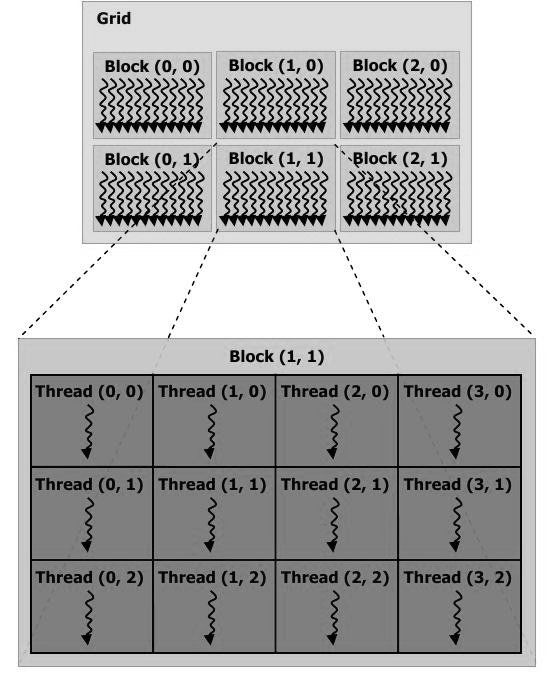
\includegraphics[width=190 pt]{gpu.jpg}
	\caption{Concurrent threads in a GPU organized in thread blocks, all of which
are running in parallel}
	\cite{pdf:NVCudaPrgGuide}
	\label{fig:gpu_diagram}
\end{figure}

\subsection{Research Objectives}

The objective of this study is to show that the GPU can be used to reduce the time
it takes to optimize game AI and thus make them more practical for use during the
development process of computer games. This research aims to illustrate the
performance gains of using a GPU to optimize the AI with the use of Genetic Algorithms.

\subsection{Research Question}

In order to complete the research objective of illustrating the benefits of using
a GPU for optimizing game AI, we will need to answer the following questions:

% research questions should be those which can't be answered through readings
% revise this as necessary.
\begin{enumerate}
 \item How do we structure the game such that most of the code may be shared between
the actual game and the offline tool that utilizes the GPU?

 \item How much faster can the GPU based application generate an optimized ``gene''
as compared to a CPU based implementation?
\end{enumerate}

\subsection{Scope and Limitations}

The focus of the study is in determining the performance gains that can be attained from
running the genetic algorithm on the GPU. The application will be a 2D tank game. The main 
variable in this study is the average running time of the application in generating 
an optimal solution. However, some parts of the code needs to be done serially, like the
genetic manipulation and the initialization. Furthermore, only the fitness process will be
parallelized.

\subsection{Significance}

Genetic algorithms have applications over a wide variety of fields.
Inspired by evolutionary biology, it can find the optimal solution
for a given problem. For example, artificial neural networks (ANN),
are used in the manufacturing industry to identify the best parameters
for constructing a model. Genetic algorithm based ANNs are found to be
the best due to its time-saving potential \cite{Venkatesan08}. Another
application can be found in the field of traffic control. They used
genetic algorithm to design an optimal toll ring scheme to reduce traffic
congestion \cite{Sumalee08}. Other applications can be found in the field
of Game AI. For example, we can make more sophisticated AI using genetic
algorithms. These AIs will be smarter in the sense that they can ``learn''.
This aspect of AI can make it more challenging, a very valuable element
in a computer game. With the age of graphics reaching its peak, the need
for better AI is starting to become an ingredient for a succesful
commercial game \cite{Yue06}. Because of the inherent ability of genetic
algorithms in learning, AIs can be made more robust. They could display
behaviors that were not seen in the previous playthrough. Thus, this
could make more challenging AIs after each playthrough. An application
of this can be seen in an experiment to create an intelligent player
for a game titled ``Megaman 2.'' Here the
computer controlled player played by trying different sets of inputs
to defeat a particular boss named ``Air Man.'' With each generation,
the computer player performed better than its previous playthrough
until it had reached the point wherein its fitness score would no longer
increase \cite{website:Kuliniewicz09}.


Various studies have already been done in the fields of genetic algorithm with
some of the applications being used commercially. However, it would seem that there
has yet to be any study done in improving genetic algorithms using the GPU for optimizing
game AI. It has been proven that genetic algorithms are limited and impractical without
the processing power of the GPU \cite{Banzhaf09}. Without this limitation however, GAs
could be used to optimize game AI in place of manually hand tuning them. Not only does
this have the potential to reduce the time it takes to fine-tune the game AI, it will
also allow the game developer/designer to work on other tasks while the computer
does the fine-tuning.

\section{Review of Related Literature}
This section aims to provide the context where this study may be placed. 
Studies that have already been made in the field are to be discussed here in order to 
explain the concepts involved in enhancing genetic algorithms through the GPU and 
genetic algorithms in a game. The section will also highlight contributions not yet 
applied in the field, namely using the GPU to enhance genetic algorithms in a game.

\subsection{Genetic Algorithms through the GPU}
\subsubsection{Genetic Algorithm Acceleration through GPU}
Genetic programming can be a very time-consuming process.  The members of its
populations are optimized against a fitness landscape through a fitness check. It
then tries the output or plugs it in again for a better fitness score. For a large
population, the processing power needed cannot be handled by the CPU alone. GPUs in
PCs are considered as more powerful in pure FLOPS \cite{Banzhaf09}.
For example, in the GeForce 8 Series the NVIDIA 8800 Ultra performs around 576 GFLOPS
on 128 processing elements. This equates to around 4.5 GFLOPS per element, compared
with 2.75 per core for the Blue Gene/L supercomputer.  With that kind of processing power, 
solving computation-intensive problems will take less time.  

A sample application can be found in the KDD 1999 IDS dataset, where, they had around
4 million entries \cite{Banzhaf09}. They evaluated 10 percent of the total subset
that were given. They found out that it only took 5.86 ms to evaluate on a GPU
compared to the 43.54 ms on the CPU. They also used genetic programming to
reverse engineer image filters, i.e., find the mapping between an image and the
output of a filter applied to it. The results were that the CPU process was 100
times slower than the GPU one. 

\subsubsection{Single Instruction, Multiple Threads Architecture of Nvidia
Graphics Card}


\begin{figure}
	\centering
		\graphicspath{{images/}}
		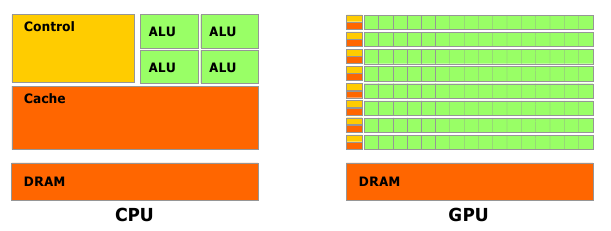
\includegraphics[width=190 pt]{cpu_gpu_blackandwhite.png}
	\caption{CPU vs GPU architecture}
	\cite{pdf:NVCudaPrgGuide}
	\label{fig:gpu_diagram}
\end{figure}

A multiprocessor creates, manages, and executes threads in groups of 32
threads \cite{pdf:NVCudaPrgGuide}. 
These group of threads are called warps. Each threads have their start at the same 
time and at the same program address. However, they have their own instruction address 
counter and register state. Thus, the threads are able to branch and execute independently.
When a multiprocessor is given one or more thread blocks to execute, it partitions into warps 
that get scheduled for execution. A warp executes one common instruction at a time. When
all 32 threads of a warp agree on their execution path, full efficiency is realized. If the threads
diverge via a data-dependent conditional branch, the warp serially executes each branch.
The threads will then converge back to the same execution path.  However, the divergence only
happens within a warp and does not affect other warps.

The single instruction, multiple threads (SIMT) architecture is similar to the single instruction,
multiple data (SIMD) vector organizations in that a single instruction controls multiple processing
elements \cite{pdf:NVCudaPrgGuide}. The difference is that the SIMD vector
organizations expose the SIMD width to the software. The SIMT instructions, on
the other hand, specify the execution and branching behavior of a single thread.
In contrast with SIMD vector machines, SIMT enables parallel coding for
independent, scalar threads, as well as data-parallel code for 
coordinated threads. 

\subsubsection{Using CUDA in Accelerating Genetic Algorithms}
Several computers can be used to efficiently process large datasets and execute complex
and evolved programs \cite{Harding09}. They used the spare processing power seen in the
computers in the student's laboratory. It detailed how a root computer distributed work
over a network of computers to increase processing speed and efficiency. Further
implementations were introduced in the field of genetic algorithms. NVIDIA introduced a new 
feature called the Compute Unified Device Architecture (CUDA),
a general-purpose parallel architecture with a new parallel programming model and instruction
set architecture \cite{Zhang09}. They present that with the given technology, genetic algorithms
are performed faster and more effectively. Because the GPU is much more effective in terms of primitive
operations, CUDA was introduced to take advantage of the massively parallel high-performance
computing on the GPU.  

\subsubsection{Implementing High Performance Genetic Programming}
However, not all genetic programs are equal in performance. Robbiliard and his colleague showed the difference between
Block genetic programming and Thread genetic programming\cite{Robbilliard09}. A Block
genetic progamming is where every genetic program is interpreted by all threads running
on a given processor. On the other hand, a Thread genetic programming is where every genetic
program is interpreted by their own thread. They performed an experiment where
the speeds at which each setup is executed are compared. The results were that the Block genetic
programs out-performed the Thread genetic programs in every benchmark, population size and
the number of fitness cases.

\subsection{Genetic Algorithms Applied in Games}
\subsubsection{Application of Genetic Programming in a Snake Game}
Genetic algorithms in games have largely been applied in solving problems relating to
Artificial Intelligence and character behavior in games. One instance of this application
is the construction of an AI for controlling the snake in a Snake game\cite{Ehlis00}.
Tobin's approach is to alter the snake's behavior based on a gene that acts as a miniature
program that gets called at every tick of the game. Given a set of helper functions that
determined if there was danger or food in certain directions of the snake's head, the
program would construct genomes that varied in the generated tree of function calls. This
tree would then determine the snake's next actions during every tick of the game. Tobin
was able to produce genomes which created snakes that could gain scores that are close to
the maximum attainable in the game.  


A different application of genetic algorithms in a mobile version of the game of snakes
was conducted by Milan Verma and Peter McOwan in their research \cite{Verma05}. Instead
of modifying the behavior of the snake in the game, they used genetic algorithms instead
for creating whole new game levels that matched the difficulty requested by the user.
Their technique was to use genomes that determined various aspects of any single game
level and then determined the level's fitness by having the level played by a synthetic
game-player. The score that the synthetic game-player obtained would then determine if
the level is too easy or too hard and levels that matched the user's wants would then be
given to the user that requested it. Their study proved successful and they were able to
deliver a mobile game that could adapt to a user's needs.

\subsubsection{AI Game Programming}
As a proof of concept, Brian Schwab attempted to enhance the AI's ability to maneuver
the player's ship in the classic game of asteroids\cite{Schwab04}. The genomes were
constructed to represent various floating point values that would dictate different
elements for decision making. These included the distance between the ship and the asteroid,
the velocity of the ship, the velocity of the asteroid, the current angle of the rotation
of the ship and more. These values, coupled with a set of predefined functions, would then
determine how the ship would evade all the asteroids in the field. Brian was able to prove
that the ship's AI can perform better when evolved through the use of genetic algorithms as
compared to hand-modifying the AI parameters and repeatedly testing the new set of values in
the game.

\subsubsection{Verlet Integration}
The Verlet integration is a way of numerically describing  the movement of an object through
time\cite{website:Bitterli09}. There are several types of Verlet integration,
Position Verlet, Velocity 
Verlet, and Leapfrog. Position Verlet gives the new position of the object by the following 
formula:

\begin{eqnarray}
P_{new}  & = &
P_{current} + 
(P_{current} - P_{old}) +
Accel * Timestep^2 \nonumber \\
P_{old} & = & P_{new} \nonumber \\
\label{Verlet}
\end{eqnarray}

The Verlet integration eliminates the need to calculate the velocity since it estimates 
the velocity using the current position and subtracting the distance with the old position. 
Through this method, the computation is fast and stable, minimizing the computational
overhead of the game. Collision detection also becomes easier with the Verlet integration.
Collision is detected by finding the new position of an object and see if it intersects with
another object.

\section{Framework}
\subsection{Definition of Terms}

There are several terms that will be used throughout this paper.
The following terms however are central to the paper and should therefore be defined clearly
to avoid any misconceptions and misunderstandings:

\begin{itemize}
 \item Graphics Processing Unit (GPU) -  A Graphics Processing Unit or GPU is a special type
of computer device that deals with the processing of graphics that will be displayed
on screen. It is similar to a Central Processing Unit or CPU in their ability to execute
a sequence of instructions over a set of data. The difference however is that while the
CPU is capable of executing a wide range of instructions, the GPU is specialized to perform
highly intensive mathematical computations and over a large set of data in a parallel manner.

 \item Genetic Algorithm (GA) - Genetic Algorithms are part of a special family of algorithms
called Stochastic Search Algorithms, also known in simple terms as randomized search. GAs
follow nature's pattern of evolution and the concept of "survival of the fittest." Given
a random set of individuals, each one is evaluated and then scored according to a fitness function.
Individuals that obtain the best scores become part of the next generation of individuals while the
rest are replaced through reproduction (mixing elements of one individual with another individual).
Eventually, only the most "fit" of individuals will be part of the final generation.

 \item Fitness function - The fitness function is the part of the genetic algorithm that ranks
an individual according to a set of arbitrary criteria. It is the score that this function
gives to an individual that determines if the said individual will be part of the next generation
or not.

 \item Individual - An individual is a representation of a possible set of parameters to a problem.
These could be variables that may be plugged into an equation or the set of timing values for an
AI agent's reaction time. Individuals may conceptually be thought of as a possible solution to a
particular problem and the correctness of the solution is determined by the fitness function.

 \item Generation - A generation, also known as a population, is a set of individuals that represent
an iteration in the algorithm. Individuals in a generation are ranked by the fitness function and then
mixed with other individuals to generate a new set of individuals through a process akin to biological
reproduction.

  \item Optimizer - For this paper, it will refer to the application that will attempt to find an
optimal set of parameters (gene) for the game AI. Two versions of this will be developed, a CPU
based optimizer which only makes use of the main processor and the GPU version, which utilizes
the GPU for the bulk of its work.

  \item Physical Time - This refers to the time as perceived in the physical world
(clock time).

\end{itemize}

\subsection{Variables of the Study}

In order to measure the success of the project, there is a need to measure several variables. These
variables will determine if utilizing the GPU is not only efficient, but also acceptable in generating
an adequate solution to the AI problem.

\begin{itemize}
 \item Running time - The time it takes for an acceptable solution can be found in a single run.
This can pertain to the time it takes for either the CPU-based or GPU-based optimizer to find an
optimal solution to a particular problem.

 \item AI Performance - How well the AI performs in playing the game and achieving the intended goals
of the game. One of the criteria is the number of scenarios the AI player manages to survive.
\end{itemize}

\section{Methodology}
% Edit this to ensure that it turns into a clear step by step process
% for replicating the research
%
% Specify the software development cycle...
% also indicate the tools used to program (hardware and software)
%
% Instruments
% Procedures
% Data Analysis (this is where statistics come in) <-- DO NOT FORGET
\subsection{Implementation Details}

\subsubsection{Application and Tools}
We have developed an evolver application which optimized the gene and a runner
application which presented the gene. Furthermore, we also have developed a CPU and
a GPU version for both applications. The first version ran the game and performed 
the genetic operations entirely on the CPU. This version of the application served 
as a benchmark on the time it took for an optimized solution to be found through 
genetic algorithms. The other version ran the game simulation on the GPU and 
the rest of the code in the CPU.


The following were the tools, libraries and systems used for developing, testing,
and analysing the data from the application:

\begin{enumerate}
  \item Fedora 14 Linux (for the operating system)
  \item gcc 4.4.4 compiler suite
  \item Boost 1.44.0 libraries
  \item Nvidia CUDA 3.2 SDK
  \item CMake 2.8 build system
  \item ClanLib 2.2.5 game engine (to be used for viewing the AI's performance)
  \item R 2.12.1 (for ANOVA data analysis)
\end{enumerate}

% We may have to use the new research comp for testing instead.
The main system used for gathering results was a Fedora 14 desktop with an 
Intel(R) Core(TM)2 Quad CPU Q9550 @ 2.83GHz for the CPU and an 
Inno3d GeForce GTX 470 (Hawk edition) for the graphics card. The CPU used 8
threads to compute for the result while the GPU used 1024 thread blocks with
32 threads per block to compute. The main system utilized for developing and 
debugging the application was a Fedora 14 laptop with an Intel Core i3 for 
the CPU and a Nvidia Geforce 310M for the GPU.


\subsubsection{Evolution Method}
The game that we used as a test bed for our AI was a simple 2D tank game.
In order to simplify the process, only a subset of the game was implemented.
The game had a single tank controlled by the AI and the objective of the AI
was to stay alive for each scenario by evading all the bullets that approached
it from fixed points on the field. The AI took note of five elements in evading the
bullets in the playing field.

\begin{enumerate}
 \item Bullet Heading - the direction of where the bullet is heading.
 \item Bullet Position - the position of the bullet in the field.
 \item Distance State - a state where the AI takes note of the distance 
of the tank and the bullets.
 \item AI Thrust - how the AI will move (move forward, move backward, or stop).
 \item AI Heading - the indented direction the AI will move among the 18
possible direction.
\end{enumerate}

We used 1024 individuals for our tank AI. An individual was tested using 54 different
scenarios. We used 18 different angles the bullets can shoot from. We also used 4
distance states. However, the bullet fired at the tank at distance state 0 is nearly
impossible to dodge in nearly all cases. This is due to the bullet being fired at a 
very close range. Therefore, we used the last 3 distance states. The evading AI will
then check for the bullet status, which includes the position, heading, and distance,
every 30 frames. The AI will recieve 1 point for every scenario it survives. Finally,
a scenario only ends when either of these 2 conditions are met:

\begin{enumerate}
 \item Evading tank gets shot.
 \item Fired bullet reaches its maximum distance and dies out.
\end{enumerate}

Genetic evolution was performed after each generation. The top 15\% of individuals
were automatically included as part of the next generation. The remaining 85\% became
the parents of the next generation through reproduction. We got two random individuals
and picked a random point in which to split the individuals. The first part of the 
first individual was then paired with the second part of the second individual to 
create a new individual. Furthermore, the second part of the first individual was
paired with the first part of the second individual to create another individual.
Lastly, each of the new individuals has a 50\% chance of mutating, i.e., a genome
in the individual will have a different value. The process is repeated for the
rest of the individuals in the lower 85\% bracket.


We used 4 different initial seeds. We ran each seed 10 times for both the CPU and 
the GPU. Furthermore, the CPU and GPU are run separately, not simultaneously. This
is due to the GPU using CPU cycles during the reproduction phase.

\subsubsection{Data Analysis}
Data was gathered by running the CPU and GPU based applications a number of
times. There are 3 kinds of data that were gathered in each run of the application.
\begin{enumerate}
  \item The seed tag.
  \item The processor tag.
  \item The time it took to finish all 54 scenarios for all individuals of 
that generation (in physical time).
\end{enumerate}
The fitness score was not considered because the results of all runs with the
same seed produced identical scores.


We used Analysis of Variance, ANOVA, to reduce getting a Type 1 error, a false
positive error. We used a two way ANOVA because the output we get, time, might
be affected by the seed or the processor or both.
$$
SS_{total} = SS_a + SS_b + SS_{ab} + SS_{error}
$$
Our null hypothesis is the speed of CPU is equal to the speed of GPU.
$$
\mu_{CPU} = \mu_{GPU}
$$
The alternative is that the speed of CPU and GPU are not equal.
$$
\mu_{CPU} \neq \mu_{GPU}
$$

\section{Results}
\subsection{Tabular Results} 
We have set the maximum amount of generations to 24, as we have observed 
that the AI often does not evolve any further after the 24th generation. The 
table \ref{table:CPU vs GPU total runtime} and 
\ref{table:CPU vs GPU total runtime part 2} contains the total time in each
run per seed for both CPU and GPU. The ANOVA test indicates that the result
we got was not a type 1 error as shown in figure \ref{fig:anova_result}.
\begin{figure}
	\centering
		\graphicspath{{images/}}
		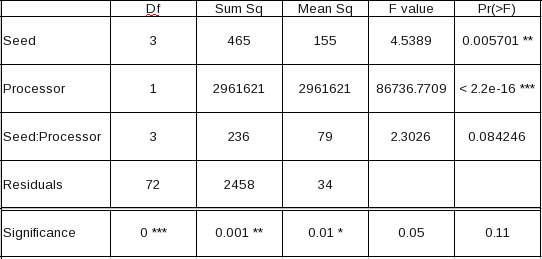
\includegraphics[width=260 pt]{Anova_Results.png}
	\caption{Anova Results}
	\label{fig:anova_result}
\end{figure}
Thus, the GPU can be considered to be faster than the CPU as shown in figure
\ref{fig:anova_result_graph}.
\begin{figure}
	\centering
		\graphicspath{{images/}}
		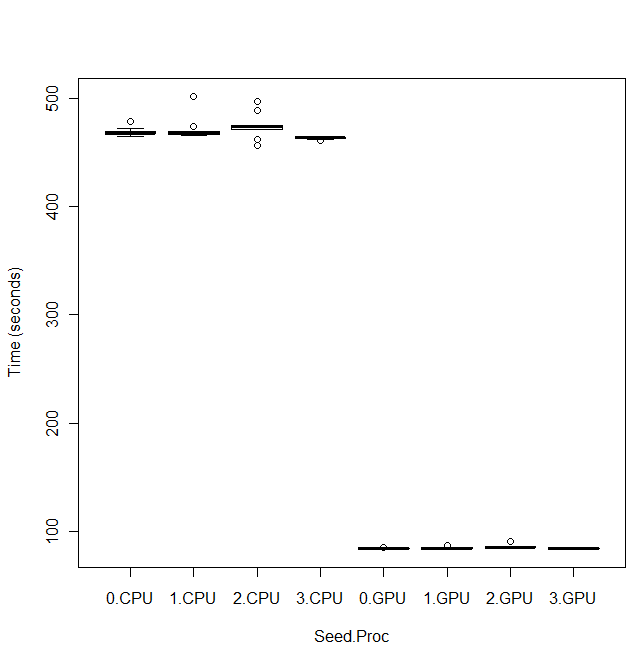
\includegraphics[width=260 pt]{Anova_Result_Graph.png}
	\caption{CPU vs GPU Graph}
	\label{fig:anova_result_graph}
\end{figure}

\begin{table}
\caption{CPU vs GPU Total Runtime Seeds 0 and 1}
\centering
 \begin{tabular}{ | l | l | l |}
    \hline
    Time & Seed & Processor \\ \hline
    471.94 & 0 & CPU \\ \hline
    469.5 & 0 & CPU \\ \hline
    468.12 & 0 & CPU \\ \hline
    468 & 0 & CPU \\ \hline
    478.42 & 0 & CPU \\ \hline
    467.59 & 0 & CPU \\ \hline
    465.22 & 0 & CPU \\ \hline
    465.5 & 0 & CPU \\ \hline
    467.64 & 0 & CPU \\ \hline
    467.19 & 0 & CPU \\ \hline
    85 & 0 & GPU \\ \hline
    83.96 & 0 & GPU \\ \hline
    84.07 & 0 & GPU \\ \hline
    83.91 & 0 & GPU \\ \hline
    83.99 & 0 & GPU \\ \hline
    83.94 & 0 & GPU \\ \hline
    83.95 & 0 & GPU \\ \hline
    83.96 & 0 & GPU \\ \hline
    83.93 & 0 & GPU \\ \hline
    83.93 & 0 & GPU \\ \hline
    469.11 & 1 & CPU \\ \hline
    466.16 & 1 & CPU \\ \hline
    466.18 & 1 & CPU \\ \hline
    468.07 & 1 & CPU \\ \hline
    465.86 & 1 & CPU \\ \hline
    466.64 & 1 & CPU \\ \hline
    467.87 & 1 & CPU \\ \hline
    468.76 & 1 & CPU \\ \hline
    473.68 & 1 & CPU \\ \hline
    501.45 & 1 & CPU \\ \hline
    83.97 & 1 & GPU \\ \hline
    84.79 & 1 & GPU \\ \hline
    83.78 & 1 & GPU \\ \hline
    83.83 & 1 & GPU \\ \hline
    83.87 & 1 & GPU \\ \hline
    83.85 & 1 & GPU \\ \hline
    83.88 & 1 & GPU \\ \hline
    83.8 & 1 & GPU \\ \hline
    86.9 & 1 & GPU \\ \hline
    86.91 & 1 & GPU \\ \hline
    \end{tabular}
\label{table:CPU vs GPU total runtime}
\end{table}

\begin{table}
\caption{CPU vs GPU Total Runtime Seeds 2 and 3}
\centering
 \begin{tabular}{ | l | l | l |}
    \hline
    Time & Seed & Processor \\ \hline
    497.14 & 2 & CPU \\ \hline
    462.1 & 2 & CPU \\ \hline
    456.83 & 2 & CPU \\ \hline
    489.04 & 2 & CPU \\ \hline
    472.8 & 2 & CPU \\ \hline
    471.66 & 2 & CPU \\ \hline
    473.58 & 2 & CPU \\ \hline
    474.54 & 2 & CPU \\ \hline
    474.99 & 2 & CPU \\ \hline
    474.22 & 2 & CPU \\ \hline
    86.13 & 2 & GPU \\ \hline
    90.46 & 2 & GPU \\ \hline
    90.48 & 2 & GPU \\ \hline
    85.75 & 2 & GPU \\ \hline
    84.77 & 2 & GPU \\ \hline
    84.96 & 2 & GPU \\ \hline
    85.06 & 2 & GPU \\ \hline
    84.92 & 2 & GPU \\ \hline
    84.96 & 2 & GPU \\ \hline
    86.18 & 2 & GPU \\ \hline
    461.94 & 3 & CPU \\ \hline
    464.13 & 3 & CPU \\ \hline
    464.6 & 3 & CPU \\ \hline
    461.13 & 3 & CPU \\ \hline
    464.12 & 3 & CPU \\ \hline
    463.9 & 3 & CPU \\ \hline
    463.06 & 3 & CPU \\ \hline
    464.25 & 3 & CPU \\ \hline
    463.54 & 3 & CPU \\ \hline
    464.36 & 3 & CPU \\ \hline
    84.22 & 3 & GPU \\ \hline
    84.27 & 3 & GPU \\ \hline
    84.24 & 3 & GPU \\ \hline
    84.24 & 3 & GPU \\ \hline
    84.27 & 3 & GPU \\ \hline
    84.25 & 3 & GPU \\ \hline
    84.2 & 3 & GPU \\ \hline
    84.23 & 3 & GPU \\ \hline
    84.28 & 3 & GPU \\ \hline
    84.22 & 3 & GPU \\ \hline
    \end{tabular}
\label{table:CPU vs GPU total runtime part 2}
\end{table}

\section{Conclusion and Recommendations}

\subsection{Conclusion}
Genetic algorithm is a powerful tool for AI creation. It can find the optimal
solution to a given problem. The only limitation it has would be the time it 
requires to produce a usable output. We proposed that using a
GPU can shorten the time it takes to generate results. We have collected the
seed, processor, and time data. The data was analysed and found that the results
were not a type 1 error, false positive error. We have proven that the GPU is faster
in manipulating game AI than the CPU.

\subsection{Recommendations}
Although we have proven that the GPU is indeed faster than the CPU, we have not
been able to optimize the code extensively for both the CPU and GPU. Possible 
optimizations for the GPU include making use of shared memory to speed up memory
accesses. On the other hand, the CPU can benefit from using intrinsics to speed
up some of the calculations.
%\end{document}  % This is where a 'short' article might terminate

%ACKNOWLEDGMENTS are optional
\section{Acknowledgments}
We would like to thank the Department of Information Systems and Computer Science of the Ateneo de
Manila University for providing funds necessary to start our research.
We would also like to thank the \textit{Sanggunian ng mga Mag-aaral ng mga Paaralang Loyola ng Pamantasang Ateneo de Manila}
for providing additional funds to purchase the needed video card. We would also like to thank
Walfrido David Diy for finding time in his schedule for thesis advice and editing. Last, but
not the least, we would like to thank Wilhansen Joseph Li for providing a way to analyse the data. 

%
% The following two commands are all you need in the
% initial runs of your .tex file to
% produce the bibliography for the citations in your paper.
\bibliographystyle{abbrv}
\bibliography{biblio}  % sigproc.bib is the name of the Bibliography in this case
% You must have a proper ".bib" file
%  and remember to run:
% latex bibtex latex latex
% to resolve all references
%
% ACM needs 'a single self-contained file'!
%
%APPENDICES are optional
%\balancecolumns
\appendix
%Appendix A
\section{Introduction}
\subsection{Background of the Study}
\subsection{Research Objectives}
\subsection{Research Question}
\subsection{Scope and Limitations}
\subsection{Significance}
\section{Review of Related Literature}
\subsection{Genetic Algorithms through the GPU}
\subsubsection{Genetic Algorithm Acceleration through GPU}
\subsubsection{Single Instruction, Multiple Threads Architecture of Nvidia
Graphics Card}
\subsubsection{Using CUDA in Accelerating Genetic Algorithms}
\subsubsection{Implementing High Performance Genetic Programming}
\subsection{Genetic Algorithms Applied in Games}
\subsubsection{Application of Genetic Programming in a Snake Game}
\subsubsection{AI Game Programming}
\subsubsection{Verlet Integration}
\section{Framework}
\subsection{Definition of Terms}
\subsection{Variables of the Study}
\section{Methodology}
\subsection{Implementation Details}
\subsubsection{Application and Tools}
\subsubsection{Evolution Method}
\subsubsection{Data Analysis}
\section{Results}
\subsection{Tabular Results} 
\section{Conclusion and Recommendations}
\subsection{Conclusion}
\subsection{Recommendations}
\section{Acknowledgments}
\section{References}

\balancecolumns
% That's all folks!
\end{document}
